
\chapter{Notes}
\section{Using Customizations}
\begin{bulletedlist}
	\item The setup function requires a named plot style drawing to be open.
	\item The setup function requires the drawing to have a plot style installed.  Use one of the drawing templates.
\end{bulletedlist}

\section{Programming and Debugging}
\begin{bulletedlist}
	\item \href{https://www.youtube.com/watch?v=Rrgx3TcXNzM}{Video on lisp debugging with GStar2023}
\end{bulletedlist}

\subsection{ZWCAD Lisp Debugging}
\subsubsection{Launch the Debugger}
\begin{numberedlist}
	\item Launch \emph{Visual Studio Code} from \emph{ZWCAD}.
	\begin{plainlist}
		\item \emph{Manage->Visual LISP Editor}
	\end{plainlist}
	\item Open the folder where the lisp files are.  This should be a location that \emph{ZWCAD} can load them.  In this case:
	\begin{plainlist}
		\item \textcode{C:\tbs{}Custom Program Files\tbs{} Support Files\tbs{}Support}
	\end{plainlist}
\end{numberedlist}


\subsubsection{Configuring}
To configure the debugger, use the following.
\begin{numberedlist}
	\item Install the ZWLisp Visual Studio Code extension.
	\item Press the \emph{Debug} button.  If there is not a \emph{launch.json} file in the folder, one will have to be created (See \figurename~\ref{fig:createlaunchjson}).
	\item Configure the debugger to point to the \emph{ZWCAD} executable (See \figurename~\ref{fig:zwcadlispsestupjson}).
\end{numberedlist}

\begin{figure}
	\centering
	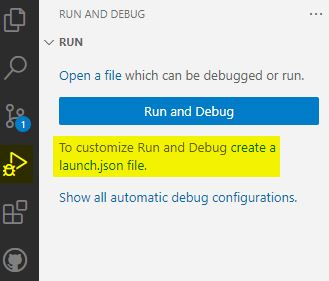
\includegraphics[width=2.5in]{createlaunchjson}
	\caption{Create a launch json for ZWCAD lisp setup.}
	\label{fig:createlaunchjson}
\end{figure}

\begin{figure}
	\centering
	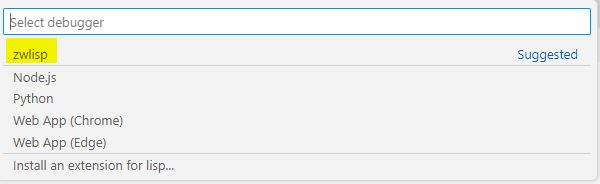
\includegraphics[width=4.5in]{selectzwlispdebugger}
	\caption{Select ZWCAD as the debugger.}
	\label{fig:selectzwlispdebugger}
\end{figure}

\begin{figure}
	\centering
	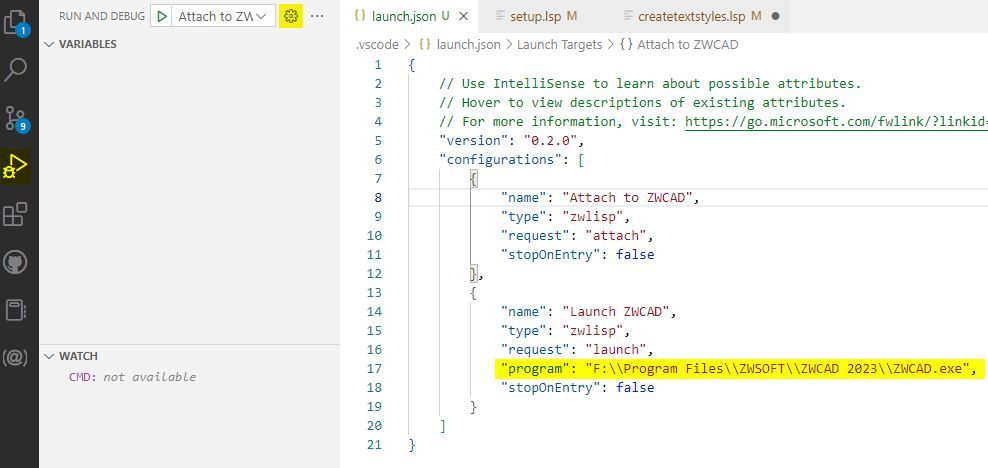
\includegraphics[width=6.5in]{zwcadlispsestupjson}
	\caption{ZWCAD lisp setup.}
	\label{fig:zwcadlispsestupjson}
\end{figure}

\subsubsection{Debugging}
To debug a lisp file, use the following.
\begin{numberedlist}
	\item Run the debugger by using the \textit{Debug} tab and clicking the \textit{Start Debugging} button.  See \figurename~\ref{fig:zwcadlispdebug}.
	\item Run the command to debug from the \emph{ZWCAD} command line.
\end{numberedlist}

\begin{figure}
	\centering
	\includegraphics[width=2.5in]{zwcadlispdebug}
	\caption{ZWCAD lisp debugging.}
	\label{fig:zwcadlispdebug}
\end{figure} 